\documentclass{ximera}
\graphicspath{
{./}
{volumes/}
{arclengths/}
{centroids/}
{techniques/}
{applications/}
{series/}
{powerseries/}
{odes/}
{lessons/}
}
\usepackage{booktabs}

\newcommand{\bigmath}[1]{$\displaystyle #1$}
\newcommand{\choicebreak}{}
\newenvironment{type}{}{}
\newenvironment{notes}{}{}
\newenvironment{keywords}{}{}
\newcommand{\offline}{}
\newenvironment{comments}{\begin{feedback}}{\end{feedback}}
\newenvironment{multiplechoice}{\begin{multipleChoice}}{\end{multipleChoice}}
\title{ODEs: Foundations}
%%%%%\author{Philip T. Gressman}

\begin{document}
\begin{abstract}
We study the fundamental concepts and properties associated with ODEs.
\end{abstract}
\maketitle

\section*{(Video) Calculus: Single Variable}
\textbf{Note: For now you can begin the video at around 1:45. We will discuss linear and separable ODEs shortly. The midpoint method and Runge-Kutta beginning around 12:15 are important things to understand, but you will not be expected to compute these yourself like you will for Euler's method.}
\youtube{UISSWvg1pg0}

\section*{Online Texts}
\begin{itemize}
\item \link[OpenStax II 4.1: ODEs]{https://openstax.org/books/calculus-volume-2/pages/4-1-basics-of-differential-equations} and \link[Direction Fields and Numerical Methods]{https://openstax.org/books/calculus-volume-2/pages/4-2-direction-fields-and-numerical-methods}
\item \link[Ximera OSU: ODEs]{https://ximera.osu.edu/mooculus/calculus2/differentialEquations/titlePage} and \link[Numerical Methods]{https://ximera.osu.edu/mooculus/calculus2/numericalMethods/titlePage}
\end{itemize}

\section*{Examples}

\begin{example}
Below you will find a slope field for the ODE $y' = -xy$.
\begin{center}
\begin{image}
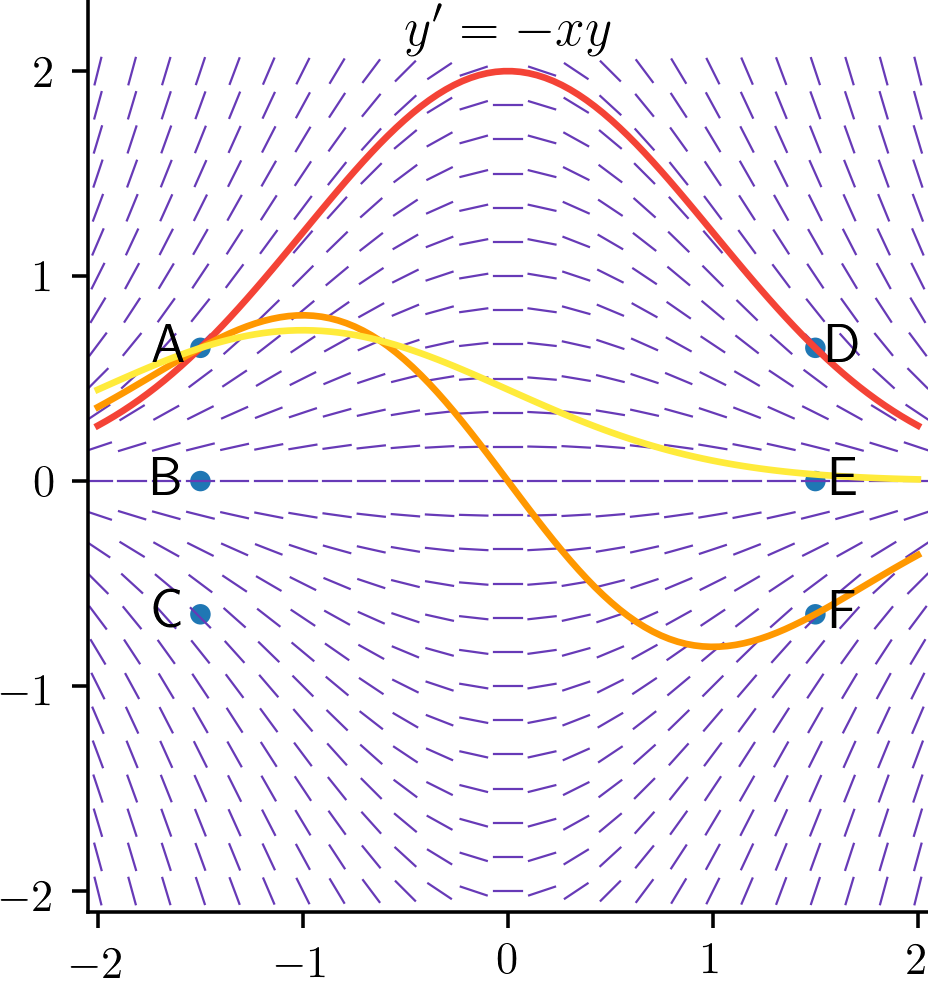
\includegraphics[width=4in]{images/slopeX01.png}
\end{image}
\end{center}
 There are three curves shown:
\[ \begin{aligned}
\text{In Red: } \ & {\displaystyle y = 2 e^{-\frac{x^2}{2}}}, \\
\text{In Orange: } \ & {\displaystyle y = -\frac{4x}{3} e^{-\frac{x^2}{2}}}, \\
\text{In Yellow: } \ & {\displaystyle y = e^{-\frac{x^2}{2} - x - \frac{3}{2}}}.
\end{aligned} \]
Which of the three curves is a solution of the ODE $y' = -xy$? In other words, which of the three curves is correctly aligned with the slope field?
\begin{multipleChoice}
\choice[correct]{Red}
\choice{Orange}
\choice{Yellow}
\end{multipleChoice}
There are also a number of points marked on the graph: point B at $(-1.5,0)$, point C at $(-1.5,-0.65)$, point D at $(1.5,0.65)$, point E at $(1.5,0)$, and point F at $(1.5,-0.65)$. The solution of the ODE which begins at the point B will pass through the point \wordChoice{\choice{D}\choice[correct]{E}\choice{F}}. Similarly, the solution which begins at C will pass through \wordChoice{\choice{D}\choice{E}\choice[correct]{F}}.
\end{example}

\begin{example}
Can two different solutions of the same first-order ODE $y' = f(x,y)$ have graphs which cross?
\begin{multipleChoice}
\choice{Yes: There are infinitely many solutions, so they can always cross.}
\choice{Yes: You can generally have many different initial conditions, so they can be arranged to cross.}
\choice{No: There is only one solution passing through any horizontal line.}
\choice[correct]{No: If there were a point of intersection, the tangent lines would be the same so the curves \\
couldn't actually cross each other there.}
\end{multipleChoice}
\end{example}

\begin{example}
The concept behind Euler's method is that we approximate a solution of an ODE of the form $y' = f(x,y)$ with a polygonal graph. Usually each segment of the graph has the same width (referred to as the \textit{step size}). We use the function $f(x,y)$ to dictate the slope of each piece of the approximation.
Let $y(x)$ be the solution to the initial value problem $y' = x +  \frac{\ln y}{\ln 2} - \frac{y}{2}$ with $y(0) = 1$.  Use Euler's Method with step size $h = 1$ to approximate the value of $y(3)$. 
\begin{itemize}
\item For this particular ODE, we have
\[ f(x,y) = \answer{ x +  \frac{\ln y}{\ln 2} - \frac{y}{2}}. \]
\item Supposing that we start at the point$x = 0$, $y = 1$, the slope will be
\[ f(0,1) = \answer{-\frac{1}{2}.} \]
\item Consider a line segment beginning at the point $(0,1)$ having slope $f(0,1)$ which you just calculated.
\begin{center}
\begin{image}
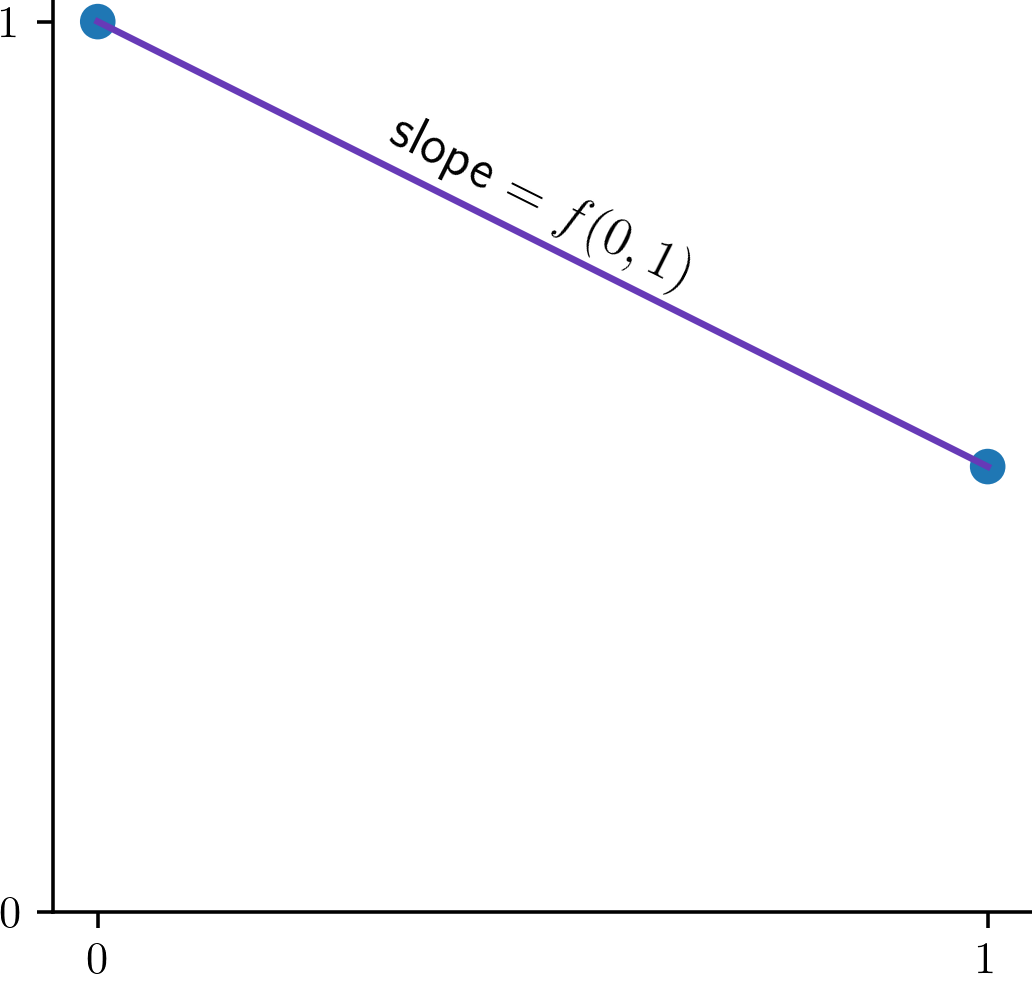
\includegraphics[width=4in]{images/euler01.png}
\end{image}
\end{center}
The line segment will pass through the point
\[ (1 , \answer{\frac{1}{2}}) \]
(use your value of $f(0,1)$ to compute a numerical value of $y$ corresponding to $x = 1$).
\item Now we repeat: Take a new line segment beginning at the point you just found. 
\begin{center}
\begin{image}
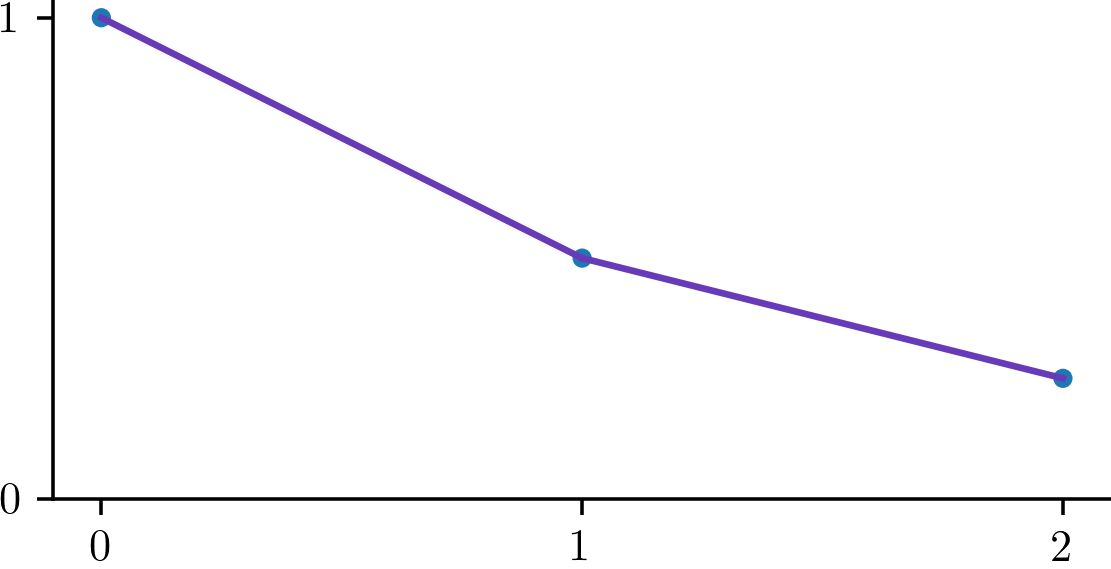
\includegraphics[width=4in]{images/euler02.png}
\end{image}
\end{center}
Its slope is given by
\[ f \left(1,\answer{\frac{1}{2}} \right)  = \answer{-\frac{1}{4}}. \]
This new line segment passes through the point $(2,\answer{1/4})$.
\item Repeat again: 
\begin{center}
\begin{image}
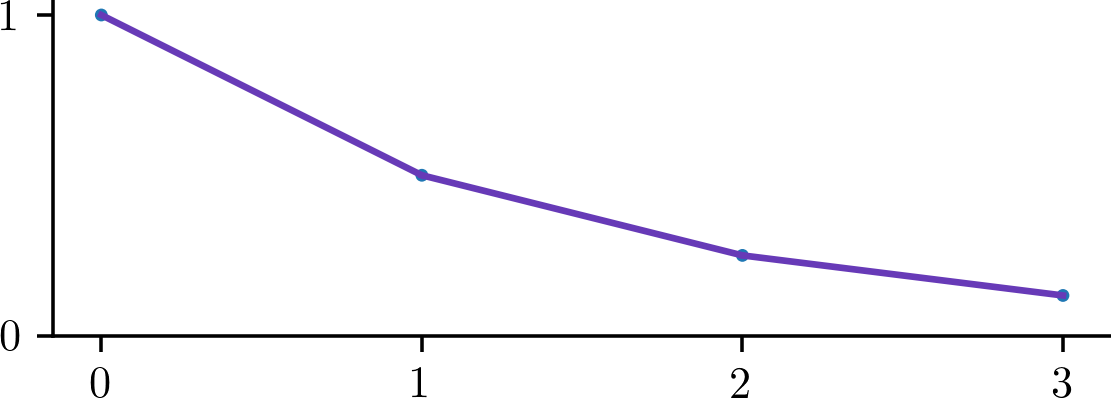
\includegraphics[width=4in]{images/euler03.png}
\end{image}
\end{center}
the line segment beginning at the point you just found will have slope
\[ f \left(2,\answer{\frac{1}{4}} \right)  = \answer{-\frac{1}{8}} \]
and will pass through the point $(3,\answer{1/8})$. Since we have arrived at an $x$-value of $3$, we may stop. The $y$-value of this most recent point is our answer:
\[ y(3) \approx \answer{\frac{1}{8}}. \]
\end{itemize}
\end{example}



\end{document}
